\begin{frame}
  \frametitle{\problemtitle}

  \begin{itemize}
  \item Given are $2\leq n\leq 12$ locations of bakeries with $0\leq x, y\leq 10^6$.
  \item We want to make a route through all $12$ of them that is as short as possible.
  \item The route follows the Manhattan distance between consecutive locations on an orthogonal grid.
  \item Choose an orientation of the grid to minimize the total length.
  \end{itemize}

  \vspace{0.5em}
  \centering
  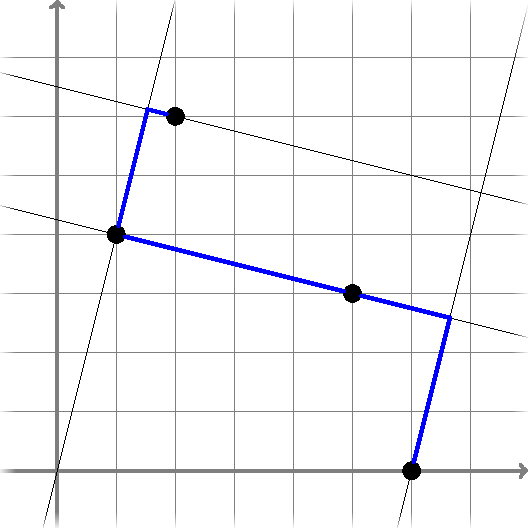
\includegraphics[width=0.30\textwidth]{sample2.pdf}

  \small
  Illustration of Sample Input 2 with a possible street layout that gives the shortest possible path that visits all bakeries in some order.
\end{frame}
